
\documentclass[a4paper,11pt]{article}
\usepackage{ifpdf}

\ifpdf
\usepackage[pdf]{graphicx}
\usepackage[pdf]{hyperref}
\else
\usepackage{graphicx}
\usepackage{hyperref}
\fi

\usepackage[svgnames]{xcolor}
\usepackage{minted}
\usepackage{amsmath}
\usepackage{amssymb}
\usepackage{xspace}
\usepackage{booktabs}
\usepackage[top=3cm, bottom=3cm, left=2.5cm,right=2.5cm]{geometry}
%\usepackage[left=3cm,right=3cm]{geometry}

\pagestyle{headings}

\author{Stuart Moodie}
\date{June 28, 2013}
\title{Proposed changes for PharmML 0.2.0}

\colorlet{bkgd}{gray!5}
%\usemintedstyle{trac}

%\newminted{xml}{bgcolor=bkgd,fontsize=\footnotesize%
%,fontfamily=courier%
%}

\newminted{xml}{fontsize=\footnotesize,fontfamily=courier}

% \newcommand{\inputxml}[1]{\inputminted[bgcolor=bkgd,fontsize=\scriptsize%
% ,fontfamily=courier%
% ]{xml}{codesnippets/#1}}

\newcommand{\cellml}{CellML\xspace}
\newcommand{\sbml}{SBML\xspace}
\newcommand{\sedml}{SED-ML\xspace}
\newcommand{\mathml}{MathML\xspace}
\newcommand{\uncertml}{UncertML\xspace}
\newcommand{\pharmml}{PharmML\xspace}
\newcommand{\xelem}[1]{\texttt{<#1>}\index{XML Element!\texttt{<#1>}}}
\newcommand{\xatt}[1]{\texttt{#1}\index{XML Attribute!\texttt{#1}}}

\begin{document}

\maketitle

\tableofcontents

\section{Introduction}

There are a number of issues we agreed that we should think about for
the next public release of \pharmml. In addition there are a number
suggestions from reviewers about changes we could make to the
language. In this document I want to highlight some issues that I
would like to see addressed and I make detailed proposals for these
changes in the spec. The proposed changes come in several forms. 1)
Refactoring of the schema design. Refactoring changes do not change
what is described by the schema and the scope and functionality of
\pharmml. 2) New features and functionality to be incorporated into
\pharmml. 3) Suggestions for larger changes to the specification that
affect the scope of \pharmml. 4) Features that we should consider, but
for which I don't have any concrete proposals.

Most of these proposals (excluding the \xatt{id} proposal in section
\ref{sec:id-prop}) have been implemented to demonstrate them and
examples 1 and 8 from the spec have been updated to use the refactored
and revised schema.

The initial version of this document was reviewed by Maciej Swat and
Niels Kristensen and I have incorporated their comments into this version.

\section{Refactoring}

\subsection{Revise the XML design principles used}

A common dilemma when designing XML documents is when do I use an
element and when an attribute? Previously when designing \pharmml we
have tended to use attributes to hold information. However, some of
these usages are at odds with design best practise, such as the guidelines provided in an IBM technical
document\footnote{\url{http://http://www.ibm.com/developerworks/xml/library/x-eleatt/index.html}}. The
advice can be summarised as follows:

\begin{description}
\item[Principle of core content] Briefly data or core content should
  be held in elements and metadata should be in attributes.
\item[Principle of structured information] If the information needs to
  be structured then it should be represented by an element. If it is
  atomic then us an attribute.
\item[Principle of readability] If the information is intended to be
  read and understood by a person then use elements. If it is intended
  to be used by a machine then use attributes.
\item[Principle of element/attribute binding] If the information to be
  represented can be modified by another attribute then use an element
  to represent it.
\end{description}

These rules are to some extent a matter of judgement and in some cases
it is not immediately clear what constitutes core content or
metadata. The names of parameters, variables and other symbols used in
\pharmml are a case in point. The names for such symbols have meaning
for a modeller, but they are also used computationally to validate the
\pharmml document. In addition, variable names can have two forms: a
computer friendly form such as \texttt{omega\_V} and a mathematical
form such as $\omega_V$. Currently \pharmml only handles the latter
form, and although this is a computational name it is also the
variable name commonly used by modellers. So if the computational name
is also the name used when discussing a model is it worth
distinguishing between the two? My proposal is to
define the identifier that is used computationally as an attribute,
but to also provide an optional `publishable' symbol name as an element. That way if
it is useful to make a distinction you can, otherwise the
computational identifier can be used as the publishable name for the
symbol. For example:
%
\begin{xmlcode}
<Variable symbID="pV" symbolType="scalar" >
  <ct:Symbol>pop_V</Symbol>
</Variable>
\end{xmlcode}

Another area where applying these design guidelines changes things is
in the way we represent numbers and other similar constructs. Instead
of using a
\xatt{value} attribute we define it using element content. So the
following:
%
\begin{xmlcode}
<ct:Scalar value="10.1"/>
<ct:Sequence begin="0" end="192" stepSize="24" />
<ct:Sequence begin="0" repetitions="2" stepSize="24" />
<ct:String value="foo"/>
\end{xmlcode}
%
becomes
%
\begin{xmlcode}
<ct:Scalar>10.1</ct:Scalar>
<ct:Sequence>
    <ct:Begin>0</ct:Begin>
    <ct:StepSize>24</ct:StepSize>
    <ct:End>192</ct:End>
</ct:Sequence>
<ct:Sequence>
    <ct:Begin>0</ct:Begin>
    <ct:StepSize>24</ct:StepSize>
    <ct:Repetitions>2</ct:Repetitions>
</ct:Sequence>
<ct:String>foo</ct:String>
\end{xmlcode}

Note that in the case of the sequence the new construct also allows us
to ensure that only a repetition or an end is defined. With the
attribute approach above this could not be validated by XML Schema
validation.

% \subsection{Define basic types in common types}

% Currently types like \xelem{Scalar} and \xelem{VarRef} are define in
% the maths schema. While this works, it make the design a messy as the
% original concept was that the maths schema was an separate module
% independent of the rest of the schema. The aim of making it modular
% was to make sure we could minimise the impact of replacing our maths
% definition with another definition, such as MathML should we wish
% to\footnote{Likewise the Uncertainty schema that describes probability
%   distributions is also modular so that we can replace it by UncertML
%   version 3.0.}.

% The proposal is that we define the basic types such as string,
% scalar\footnote{See later proposal about numerical types.} and
% Booleans as common types.

\subsection{Different Numerical Types}

Currently there is a single type for a number called the scalar. The
idea is that a scalar type can be any numerical value and the term
scalar is used to distinguish it from an array type (which we don't
have, but could do it in the future). However, in some cases it is
useful to distinguish between integer and real numbers in
\pharmml. For example, when defining a sequence the number of
repetitions should be an integer (actually a positive integer) or when
specifying the number of individuals in a Trial Design Group.

My proposal is that we have two numerical literal elements \xelem{Int}
and \xelem{Real}. These would work as follows:

\begin{xmlcode}
<ct:Int>10</ct:Scalar>
<ct:Int>-210</ct:Scalar>
<ct:Real>22.2</Real>
<ct:Real>1.5636e-36</ct:Real>
<ct:Real>.0273626</ct:Real>
<ct:Real>-2.03</ct:Real>
<ct:Real>INF</ct:Real>
\end{xmlcode}

There is a question whether we should define the element as
\xelem{Double} instead of \xelem{Real}. Ideally the \xelem{Real}
element would define an architecture independent real number with
arbitrary precision. However, applications that use such numbers will
typically use a double numerical type. Therefore we should define the
\xelem{Real} element to be an XML Schema double type, which conforms
to the IEEE double-precision 64-bit floating point type standard used
by many programming languages. This begs the question of whether we
should rename the \xelem{Real} element to be \xelem{Double} as this
matches the computational representation of the number and so makes it
clear to the user of \pharmml. An argument against this is that we are
only providing one Real type; so we don't need to distinguish between
a double and a float for example. Likewise, if we decide to change the
underlying type of \xelem{Real}, for example from double to a float,
then this change would not require a change at the XML level and the
name would not be mislead, as it would if we called the element
\xelem{Double}. On balance my preference is to use the element name
Real.

\subsection{Symbol Definition Refactored}

The current definition of \xelem{SymbolDefinition} needs tidying
up. The SymbolDefinition is now really a mechanism for defining
functions while originally I had the idea of using it to define
constants and there was a parallel element that referred to an
external definition of symbols and functions. Therefore, it makes
sense to rename it to \xelem{FunctionDefinition} and to reorganise it
slightly. The current version looks like this:
%
\begin{xmlcode}
<SymbolDefinition symbId="constantErrorModel" symbolType="scalar">
    <FunctionDefinition>
        <FunctionArgument symbId="a" symbolType="scalar"/>
        <Definition>
            <Equation xmlns="http://www.pharmml.org/2013/03/Maths" writtenVersion="0.1">
                <Var symbId="a"/>
            </Equation>
        </Definition>
    </FunctionDefinition>
</SymbolDefinition>
\end{xmlcode}
%
I propose to restructure it so that it looks like this:
%
\begin{xmlcode}
<FunctionDefinition xmlns="http://www.pharmml.org/2013/03/CommonTypes"
    symbId="constantErrorModel" symbolType="real">
    <FunctionArgument symbId="a" symbolType="real"/>
    <Definition>
        <Equation xmlns="http://www.pharmml.org/2013/03/Maths" writtenVersion="0.1">
            <Var symbId="a"/>
        </Equation>
    </Definition>
</FunctionDefinition>
\end{xmlcode}
%
As well as renaming it I propose to move the definition into the
common types schema. It is currently in the top-level pharmML schema.
  
\subsection{Change Variability Levels to be Declarative}

Currently the order of a variability level definition is used to
specified the hierarchy of variability levels. So for example to
define BSV and IOV we define the IOV level first then the BSV level
next, as below:
%
\begin{xmlcode}
<VariabilityLevel id="iov1"/>
<VariabilityLevel id="indiv"/>
\end{xmlcode}

As was pointed out by Duncan Edwards this is actually an imperative
definition as the ordering the elements are read in is important. He
suggested we make the hierarchy definition explicit and on reflection
I think he is right. Therefore I propose we change the definition to
the following:
%
\begin{xmlcode}
<VariabilityModel id="model">
    <Level symbId="indiv"/>
    <Level symbId="iov1">
        <ParentLevel>
            <ct:SymbRef symbId="indiv"/>
        </ParentLevel>
    </Level>
</VariabilityModel>
\end{xmlcode}

Here each level defines it's parent level explicitly and the topmost
level has no parent defined. It is important to note that the order is
now not significant so the following definition is equivalent to the
one above:
%
\begin{xmlcode}
<VariabilityModel id="model">
    <Level symbId="iov1">
        <ParentLevel>
            <ct:SymbRef symbId="indiv"/>
        </ParentLevel>
    </Level>
    <Level symbId="indiv"/>
</VariabilityModel>
\end{xmlcode}
%
The other thing to note is that the variability levels are now held in
a block. This is consistent with the other models in
\xelem{ModelDefinition} and this feature may be useful later when we
think about defining the variability of the residual error model.

\subsection{Improving the definition of a variable}

Applying the attribute/element design guidelines above we can refactor
the way a variable definition is designed in \pharmml. There are two main
changes. One is the way we define derivative variables (see below) and
the other is the way we indicate assignment. The example below shows the
changes:
%
\begin{xmlcode}
<ct:Variable symbId="k" symbolType="real">
    <ct:Symbol>k</ct:Symbol>
    <ct:Description>This is a description.</ct:Description>
    <ct:Assign>
        <Equation xmlns="http://www.pharmml.org/2013/03/Maths" writtenVersion="0.1">
            <Binop op="divide">
                <Var block="p1" symbId="Cl"/>
                <Var block="p1" symbId="V"/>
            </Binop>
        </Equation>
    </ct:Assign>
</ct:Variable>
\end{xmlcode}
%
The \xelem{Symbol} and \xelem{Description} elements are optional. We
use an \xelem{Assign} element to indicate where the RHS of the
assignment is. This is optional --- a variable does not need to be
assigned when it is defined. We could strictly do without the
\xelem{Assign} element but it makes the design cleaner and reduces
redundancy as we reference a global \xelem{Assign} element defined in
the Common Types schema. This makes it simpler to parse the model as standard
syntactic patterns are reused throughout the language.

\subsection{Improving the definition of a derivative}

Currently we use the type to define whether a variable is a
derivative. While this works it is not strictly correct as the type of
the variable is a scalar \emph{and} the variable is also a
derivative. While at the moment this does not matter, the current
approach is not easily extensible. For example it may be useful in the
future to provide derivatives for variables with types not yet
supported, such as vectors. In addition, the independent variable is
defined as an attribute that should only be defined if the variable is
a derivative. This is a rule that cannot be enforced by XML schema
validation directly. However, after refactoring to an element is can
be. The example below shows the current approach:
%
\begin{xmlcode}
<Variable symbId="x" independentVar="t" symbolType="derivative">
    <Equation xmlns="http://www.pharmml.org/2013/03/Maths" writtenVersion="0.1">
      <!-- Snip -->
    </Equation>
</Variable>
\end{xmlcode}
%
and how the same definition would look under this proposal:
%
\begin{xmlcode}
<ct:DerivativeVariable symbId="x" symbolType="real">
    <ct:Description>Concentration</ct:Description>
    <ct:Assign>
        <Equation xmlns="http://www.pharmml.org/2013/03/Maths" writtenVersion="0.1">
          <!-- Snip -->
        </Equation>
    </ct:Assign>
    <ct:IndependentVariable>
        <ct:SymbRef symbId="t"/>
    </ct:IndependentVariable>
    <ct:InitialCondition>
       <ct:Real>0</ct:Real>
    </ct:InitialCondition>
</ct:DerivativeVariable>
\end{xmlcode}

By using the \xelem{ct:DerivativeVariable} element we can now enforce
the rule that the independent variable can only be defined for a
derivative variable. Note that the type of the variable is defined
using the \xatt{symbolType} attribute, which has it's value fixed to
`real'. We do this because \pharmml only supports derivative variables
of that type, but providing the attribute enables future modification
and makes the XML self-documenting. The final change of note is that
the initial condition is now associated with the
derivative. Previously this was a completely separate element, but by
making it part of the derivative we ensure that only derivative
variables are provided with initial conditions.

\subsection{Improving the definition of a variable assignment}

The refactoring of the assignment follows the element vs attribute
design principle described above and aims to be consistent with the
variable declaration. See the example:
%
\begin{xmlcode}
<ct:VariableAssignment>
    <ct:SymbRef  block="c1" symbId="omega_W"/>
    <ct:Description>This is the: c1.omega_W = 1409/100</ct:Description>
    <ct:Assign>
        <math:Equation writtenVersion="0.1">
            <!-- 1409/100 = 14.09 -->
            <math:Binop op="divide">
                <math:Scalar>1409</math:Scalar>
                <math:Scalar>100</math:Scalar>
            </math:Binop>
        </math:Equation>
    </ct:Assign>
</ct:VariableAssignment>
\end{xmlcode}
%
The \xelem{VariableAssignment} is defined as a common type and is
reused in several places throughout the schema.

\subsection{Reusing common elements}

In the current version of \pharmml we have a schema called
commonTypes.xsd where we put commonly used types such as variable
references, sequences, vectors etc. The idea is that this schema holds
common types and structures that are used in common by the other
schemas (except Math.xsd and Uncertainty.xsd). This helps us remove
redundancy in the design and makes changing and extending the schema
easier. During the refactoring I propose to extend this approach and
put reusable elements into the common schema. Elements such as String,
SymbRef, VariableAssignment etc are defined here as global elements
that can then be referenced by the other schemas. In addition to
further reducing redundancy this approach also promotes the reuse of
the same constructs throughout the language which simplifies parsing
and validation of the language.

To help with this some elements in the current \pharmml spec are being
replaced with a common reference. In particular the
\xelem{initialAssignment} element in the simulation and estimation
step is being replaced with a reference to the
\xelem{VariableAssignment} element and the variable declarations in
the \xelem{ModellingSteps} and \xelem{StructuralModel} elements are
each replaced by the VariableAssignment.

% \subsection{Restrict RHS to scalar types}

% In the current spec, largely for historical reasons, the
% right-hand-side of an equation could contain non-scalar types such as
% a distribution, a vector or a sequence. Incompatible types would get
% caught by type checking but it doesn't make sense to keep these
% structures as they will always fail. Therefore, the schema has been
% changed so that only scalar structures are allowed on the RHS of an
% scalar quantity.


\section{New or Modified Functionality}

\subsection{Element identifier for annotation?}
\label{sec:id-prop}

Our current idea of how to link annotation (aka metadata) to a
\pharmml document is to use xpath to point from the ontology terms to
the elements in the XML document. While this will work and be very
flexible I am not clear how we will be able to map from the XML
structures identified to the software API. For example, if we want to
annotate a variable definition the xpath definition would identify the
\xelem{VariableDefinition} element containing this definition. In
software we would need to find this element in the XML and then map
from this element to a corresponding Java class in libPharmML. This
may be possible, but an alternate way to do the same thing would be to
write an xpath that points to the \xatt{symbID} attribute of the same
element. Getting the software to recognise that these are essentially
the same may be difficult. We need to explore this by testing to be
sure, but an alternate mechanism may be to provide all elements with a
unique identifier, an \xatt{id} attribute. If this was mandatory for
all elements then you could guarantee that all elements in the
\pharmml document are annotatable. The \xatt{id} would also be an
attribute in the Java class so the mapping between annotation and
PharmML could be carried out directly at the software level. This is a
stricter form of the approach taken by SBML, which uses a
\xatt{metaid} attribute that is optional. SBML uses \xatt{metaid}
because the \xatt{id} attribute was originally used to define variable
names. The \xatt{id} convention is consistent with other XML schemes
such as MathML and XML-RDF. Making it mandatory means that we don't
have to change the \pharmml document in order to annotate it, because
all elements are guaranteed to have an identifier that can be
referenced. Incidentally, this approach will be much more effective
after the refactoring ideas described above are implemented because
the elements of information that we may want to annotate are stored as
XML elements whereas in some cases they are currently represented as
XML attributes.

Below is a code snippet illustrating how this identifier would work:

\begin{xmlcode}
<FixedEffect id="e10" symbId="beta_V">
    <Covariate id="e11" >
        <ct:SymbRef id="e12" symbId="W"/>
    </Covariate>
</FixedEffect>
<FixedEffect id="e13" symbId="beta_Cl">
    <Covariate id="e14">
        <ct:SymbRef id="e15" symbId="W"/>
    </Covariate>
</FixedEffect>
<RandomVariable id="e16" symbId="eta_V">
    <ct:VariabilityReference id="e17">
        <ct:SymbRef id="e18"  block="model" symbId="level"/>
   </ct:VariabilityReference>
\end{xmlcode}

\subsection{Remove the assumptions in the model definition}

\subsubsection{Improved Parameter Model}

The parameter model can be expressed in three forms:

\begin{align*}
\intertext{Type 1. (implicit) equation type of parameter model}
\psi_i &= H(\beta, c_i, \eta_i)
\intertext{Type 2. Gaussian model with general covariate model}
h(\psi_i) &= H(\beta, c_i) + \eta_i
\intertext{Type 3. Gaussian model with linear covariate model}
h(\psi_i) &= h(\psi_{pop}) + \beta c_i + \eta_i
\end{align*}
with:
\begin{itemize}
\item individual parameter, $\psi_i$
\item population parameter, $\psi_{\textit{pop}}$
\item random effect, $\eta_i$
\item fixed effects, $\beta$
\item arbitrary function , $H$
\item function which transforms the model on both sides, $h$
\end{itemize}




\subsubsection{Linear Parameter Model Assumptions}

As is made clear in the mathematical representation section of the
spec, we currently assume linear model for parameter definitions in
\pharmml such as the following\footnote{This is taken verbatim from
  the current \pharmml specification.}:

\begin{align}
h(X_i) &= h(X_{typical}) + \underbrace{\beta C_i}_{\text{\parbox{2cm}{\centering linear covariate\\[-4pt] model}}} + \underbrace{\eta_i^{(0)}+ \eta_{ik}^{(-1)} + \dots}_{\text{\parbox{3cm}{\centering IIV and other\\[-4pt] levels of variability}}} \label{eqn:standard-param-eqn}
\end{align} 

According to its additive structure a model for an individual parameter consists of
\begin{itemize}
\item
parameter transformation, $h$
\item
population/typical value of the parameter, $X_{typical}$
\item
linear covariate model, $\beta C_i$, with
\begin{itemize}
\item
fixed effects, $\beta$
\item
categorical or continuous covariates, $C_i$, e.g. \textit{Sex} or \textit{Weight}
\end{itemize}
\item
random effects, $\eta$'s, \textit{inter-individual/occasion} and other levels of variability with $\eta$'s for every level being 
\end{itemize}

There was considerable feedback from reviewers and at the last
consortium meeting this approach was too restrictive and that we
should eliminate these assumptions. The aspiration for many was that
\pharmml could encode all models that could be defined in NMTRAN. The
issue for me is to try and do this in a way that allows us to identify
the components of the parameter model while providing this
flexibility.

\paragraph{The Simple Case}

My proposal is to split out the parameter definition into its
component parts by making a random variable a first class element. So
to encode the following expression:
%
\begin{align}
\log(ka_{i}) &=  \log(pop_{ka}) + \eta_{ka,i}
\end{align}
%
we can define it in XML as follows:
%
\begin{xmlcode}
<RandomVariable levelId="indiv" symbId="eta_ka">
    <Distribution xmlns="http://www.pharmml.org/2013/03/Uncertainty"
      writtenVersion="0.1">
        <Normal>
          <!-- snip -->
        </Normal>
    </Distribution>
</RandomVariable>
<Parameter symbId="ka">
    <LhsTransformation>log</LhsTransformation>
    <ct:Assign>
        <Equation xmlns="http://www.pharmml.org/2013/03/Maths" writtenVersion="0.1">
            <Binop op="plus">
                <Uniop op="ln">
                    <Var symbId="pop_ka"/>
                </Uniop>
                <Var symbId="eta_ka"/>
            </Binop>
        </Equation>
    </ct:Assign>
</Parameter>
\end{xmlcode}
%
Thus we are clear what is the random variable and the paramete, but their relationship is defined explicitly.


\paragraph{The covariate model: incorporating fixed effects to a continuous covariate}

 Next we incorporate the covariate and fixed effects to define the following:
%
\begin{align}
\log(V_i) &= \log(\mathrm{pop_{V}}) + \beta_{1,V}\log(W_i/70) + \eta_{V,i}
\end{align}
%
We define this in XML by defining the fixed effect parameters, the random
variable and then the parameter which incorporates these elements into
the above equation.
%
\begin{xmlcode}
<Parameter symbId="pop_V"/>
<Parameter symbId="omega_V"/>
<Parameter symbId="beta_V"/>
<RandomVariable levelId="indiv" symbId="eta_V">
    <Distribution xmlns="http://www.pharmml.org/2013/03/Uncertainty"
      writtenVersion="0.1">
        <Normal>
           <!-- snip -->
        </Normal>
    </Distribution>
</RandomVariable>
<Parameter symbId="V">
    <LhsTransformation>log</LhsTransformation>
    <ct:Assign>
        <Equation xmlns="http://www.pharmml.org/2013/03/Maths" writtenVersion="0.1">
            <Binop op="plus">
                <Uniop op="ln">
                    <Var symbId="pop_V"/>
                </Uniop>
                <Binop op="plus">
                    <Binop op="times">
                        <Var symbId="beta_V"/>
                        <Var block="c1" symbId="W"/>
                    </Binop>
                    <Var symbId="eta_V"/>
                </Binop>
            </Binop>
        </Equation>
    </ct:Assign>
</Parameter>
\end{xmlcode}

\paragraph{Alternate equivalent definitions}

As pointed out in Marc Lavielle's document\footnote{``Mathematical
  description of mixed effects models.'' Marc Laveille June 2012.}
there are other ways to define a parameter equivalent to that
described in equation \ref{eqn:standard-param-eqn}. For example the
following is typically\footnote{The parameters $\mathrm{pop}_V$ and
  $\beta_V$ might be merged into a single parameter in this case, but
  they are kept here for consistency with previous examples.} how a
parameter would be defined in NONMEM:
%
\begin{align*}
V_i &= pop_{V} \cdot \beta_{1,V} \cdot \log(W_i/70) \cdot
\exp\left(\eta_{V,i} \right)
\end{align*}
%
and this can now be encoded (without transforming it into the form in
equation \ref{eqn:standard-param-eqn} as:
%
\begin{xmlcode}
<Parameter symbId="pop_V"/>
<Parameter symbId="omega_V"/>
<Parameter symbId="beta_V"/>
<RandomVariable symbId="eta_V">
    <ct:VariabilityReference>
        <ct:SymbRef block="model" symbId="indiv"/>
    </ct:VariabilityReference>
    <Distribution xmlns="http://www.pharmml.org/2013/03/Uncertainty" writtenVersion="0.1">
        <Normal>
            <Mean>
                <Scalar
                xmlns="http://www.pharmml.org/2013/03/Maths">0</Scalar>
            </Mean>
            <StdDev>
                <Var xmlns="http://www.pharmml.org/2013/03/Maths"
                symbId="omega_V"/>
            </StdDev>
        </Normal>
    </Distribution>
</RandomVariable>
<Parameter symbId="V">
    <ct:Assign>
        <Equation xmlns="http://www.pharmml.org/2013/03/Maths" writtenVersion="0.1">
            <Binop op="times">
                <Var symbId="pop_V"/>
                <Binop op="times">
                    <Var block="c1" symbId="W"/>
                    <Uniop op="exp">
                        <Var symbId="eta_V"/>
                    </Uniop>
                </Binop>
            </Binop>
        </Equation>
    </ct:Assign>
</Parameter>
\end{xmlcode}


\paragraph{The covariate model: incorporating categorical covariates}

We of course have to extend this approach to deal with categorical
covariates. In this case we use a piecewise function to set a flag
variable \texttt{one\_ka\_treatseq} that can be incorporated into the main
parameter equation. We do this using a piecewise function as follows:

\begin{xmlcode}
<Parameter symbId="one_ka_treatseq">
    <ct:Symbol>1_ka_treatset</ct:Symbol>
    <ct:Assign>
        <math:Equation writtenVersion="0.1">
            <math:Piecewise>
                <math:Piece>
                    <math:Scalar>1</math:Scalar>
                    <math:Condition writtenVersion="0.1">
                        <math:LogicBinop op="eq">
                            <math:Var block="c1" symbId="W"/>
                            <math:String value="AB"/>
                        </math:LogicBinop>
                    </math:Condition>
                </math:Piece>
                <math:Piece>
                    <math:Scalar>0</math:Scalar>
                    <math:Condition writtenVersion="0.1">
                        <math:Otherwise/>
                    </math:Condition>
                </math:Piece>
            </math:Piecewise>
        </math:Equation>
    </ct:Assign>
</Parameter>
\end{xmlcode}
which is equivalent to:
%
\begin{align*}
1_{\mathrm{ka,TreatSeq}_i=\mathrm{A-B}} &=
\begin{cases}
1 & \text{if } W \text{ has category } \mathrm{A-B}\\
0 & \text{otherwise}
\end{cases}
\intertext{We can incorporate this into the full parameter definition:}
\log(ka_{i}) &= \log(ka_{pop}) + \beta_{ka,TreatSeq}1_{TreatSeq_i=\mathrm{A-B}} + \eta_{ka,i}
\end{align*}
%
which gives the following equivalent XML definition:
%
\begin{xmlcode}
<Parameter symbId="ka">
    <LhsTransformation>log</LhsTransformation>
    <ct:Assign>
        <Equation xmlns="http://www.pharmml.org/2013/03/Maths" writtenVersion="0.1">
            <Binop op="plus">
                <Uniop op="log">
                    <Var symbId="pop_ka"/>
                </Uniop>
                <Binop op="plus">
                    <Binop op="times">
                        <Var symbId="beta_ka_treatseq"/>
                        <Var symbId="one_beta_ka_treatseq"/>
                    </Binop>
                    <Var symbId="eta_ka"/>
                </Binop>
            </Binop>
        </Equation>
    </ct:Assign>
</Parameter>
\end{xmlcode}

\paragraph{Non linear parameter models}

These changes now allow us to describe more complex parameter
models. For example the following is taken from the NONMEM User
Manual\footnote{NONMEM Users Guide - Part V: Introductory Guide, p 34.}
and describes a parameter fixed effect with a saturation model as follows:
%
\begin{align*}
\mathrm{\widetilde{CL}}_{\mathrm{met}} &= W \left(\Theta_1 - \left(\frac{\Theta_2 \mathrm{Cpss_2}}{\Theta_3 + \mathrm{Cpss}_2}\right)\right)
\end{align*}
%
Because there are no assumptions in our parameter model we can express
this equation explicitly in the RHS of the parameter assignment. This
can be represented in \pharmml as follows:
%
\begin{xmlcode}
<Parameter symbId="CL_met">
    <Assign xmlns="http://www.pharmml.org/2013/03/CommonTypes">
        <Equation xmlns="http://www.pharmml.org/2013/03/Maths"
          writtenVersion="0.1">
            <Binop op="times">
                <Var block="c1" symbId="W"/>
                <Binop op="minus">
                    <Var symbId="theta1"/>
                    <Binop op="divide">
                        <Binop op="times">
                            <Var symbId="theta2"/>
                            <Var symbId="Cpss2"/>
                        </Binop>
                        <Binop op="plus">
                            <Var symbId="theta3"/>
                            <Var symbId="Cpss2"/>
                        </Binop>
                    </Binop>
                </Binop>
            </Binop>
        </Equation>
    </Assign>
</Parameter>
\end{xmlcode}

In another example, this time of an individual parameter definition,
I've taken an example from Hooker \emph{et al.} 2008\footnote{ Hooker
  et al. ``Population Pharmacokinetic Model for Docetaxel in Patients
  with Varying Degrees of Liver Function: Incorporating Cytochrome
  P450 3A Activity Measurements'' Clinical Pharmacology \& Therapeutics
  84, 111-118 (July 2008) \textbar
  \url{doi:10.1038/sj.clpt.6100476}}. We describe unbound plasma
clearance using the individual parameter $\mathit{CL}_i$ as follows:
%
\begin{align*}
\mathrm{CL}_i &=
\begin{cases}
\eta_{\mathrm{CL}} \cdot \mathrm{CL}_{\mathrm{normal\, LF}} \cdot f_{\mathrm{BSA}} \cdot
f_{\mathrm{AAG}} \cdot f_{\mathrm{ERMBT, normal\, LF}} & \text{if } \mathrm{LFG} = 1\\
\eta_{\mathrm{CL}} \cdot \mathrm{CL}_{\mathrm{impaired\, LF}} \cdot f_{\mathrm{BSA}} \cdot
f_{\mathrm{AAG}} \cdot f_{\mathrm{ERMBT, impaired\, LF}} & \text{if } \mathrm{LFG}
> 1
\end{cases}\\
f_{\mathrm{BSA}} &= \mathrm{BSA} / \overline{\mathrm{BSA}}\\
f_{\mathrm{AAG}} &= 1 + \theta_{\mathrm{AAG-CL}} \cdot \left(\mathrm{AAG} / \overline{\mathrm{AAG}}\right)\\
f_{\mathrm{ERMBT, normal\, LF}} &= 1 + \theta_{\mathrm{ERMBT, normal\, LF}} \cdot
\left(\mathrm{ERMBT} - \overline{\mathrm{ERMBT}}_{\mathrm{normal\, LF}}\right)\\
f_{\mathrm{ERMBT, impaired\, LF}} &= 1 + \theta_{\mathrm{ERMBT, impaired\, LF}} \cdot
\left(\mathrm{ERMBT} - \overline{\mathrm{ERMBT}}_{\mathrm{impaired\, LF}}\right)
\end{align*}
%
With the proposed changes to the paramater model this can be encoded
as follows:
%
\begin{xmlcode}
<Parameter symbId="f_ERMBT_normalLF">
    <ct:Assign>
        <Equation xmlns="http://www.pharmml.org/2013/03/Maths" writtenVersion="0.1">
            <Binop op="plus">
                <Scalar>1</Scalar>
                <Binop op="times">
                    <Var symbId="theta_ERMBT_normalLF"/>
                    <Binop op="minus">
                        <Var symbId="ERMBT"/>
                        <Var symbId="ERMBT_normalLF"/>
                    </Binop>
                </Binop>
            </Binop>
        </Equation>
    </ct:Assign>
</Parameter>
<Parameter symbId="theta_ERMBT_impairedLF"/>
<Parameter symbId="f_ERMBT_impairedLF">
    <ct:Assign>
        <Equation xmlns="http://www.pharmml.org/2013/03/Maths" writtenVersion="0.1">
            <Binop op="plus">
                <Scalar>1</Scalar>
                <Binop op="times">
                    <Var symbId="theta_ERMBT_impairedLF"/>
                    <Binop op="minus">
                        <Var symbId="ERMBT"/>
                        <Var symbId="ERMBT_impairedLF"/>
                    </Binop>
                </Binop>
            </Binop>
        </Equation>
    </ct:Assign>
</Parameter>
<Parameter symbId="theta_AAG_CL"/>
<Parameter symbId="f_AAG">
    <ct:Assign>
        <Equation xmlns="http://www.pharmml.org/2013/03/Maths" writtenVersion="0.1">
            <Binop op="plus">
                <Scalar>1</Scalar>
                <Binop op="times">
                    <Var symbId="theta_AAG_CL"/>
                    <Binop op="minus">
                        <Var symbId="AAG"/>
                        <Var symbId="AAG_bar"/>
                    </Binop>
                </Binop>
            </Binop>
        </Equation>
    </ct:Assign>
</Parameter>
<Parameter symbId="f_BSA">
    <ct:Assign>
        <Equation xmlns="http://www.pharmml.org/2013/03/Maths" writtenVersion="0.1">
            <Binop op="divide">
                <Var symbId="BSA"/>
                <Var symbId="BSA_bar"/>
            </Binop>
        </Equation>
    </ct:Assign>
</Parameter>
<RandomVariable symbId="eta_CL">
    <ct:VariabilityReference>
        <ct:SymbRef symbId="indiv"/>
    </ct:VariabilityReference>
    <Distribution xmlns="http://www.pharmml.org/2013/03/Uncertainty"
    writtenVersion="0.1">
         <!-- Snip -->
    </Distribution>
</RandomVariable>
<Parameter symbId="CL">
    <ct:Assign>
        <Equation xmlns="http://www.pharmml.org/2013/03/Maths" writtenVersion="0.1">
            <Piecewise>
                <Piece>
                    <Binop op="times">
                        <Uniop op="exp"><Var symbId="eta_CL"/></Uniop>
                        <Binop op="times">
                            <Var symbId="CL_normalLDF"/>
                            <Binop op="times">
                                <Var symbId="f_BSA"/>
                                <Binop op="times">
                                    <Var symbId="f_AAG"/>
                                    <Var symbId="f_ERMBT_normalLF"/>
                                </Binop>
                            </Binop>
                        </Binop>
                    </Binop>
                    <Condition writtenVersion="0.1">
                        <LogicBinop op="eq">
                            <Var symbId="LFG"/>
                            <Scalar>1</Scalar>
                        </LogicBinop>
                    </Condition>
                </Piece>
                <Piece>
                    <Binop op="times">
                        <Uniop op="exp">
                            <Var symbId="eta_CL"/>
                        </Uniop>
                        <Binop op="times">
                            <Var symbId="CL_impairedLF"/>
                            <Binop op="times">
                                <Var symbId="f_BSA"/>
                                <Binop op="times">
                                    <Var symbId="f_AAG"/>
                                    <Var symbId="f_ERMBT_impairedLF"/>
                                </Binop>
                            </Binop>
                        </Binop>
                    </Binop>
                    <Condition writtenVersion="0.1">
                        <LogicBinop op="gt">
                            <Var symbId="LFG"/>
                            <Scalar>1</Scalar>
                        </LogicBinop>
                    </Condition>
                </Piece>
            </Piecewise>
        </Equation>
    </ct:Assign>
</Parameter>
\end{xmlcode}


These changes preserve the information we capture in the
current version of \pharmml, but provide much more flexibility because
we eliminate the assumptions and separate out the definition of the
random variable from that of the parameter.


\subsubsection{Residual Error Model}

The residual error model is define as part of the observation
model. Currently we assume the following structure\footnote{This is
  reproduced verbatim from the \pharmml specification.}, where the
equation below defines a general nonlinear mixed effects model for
continuous data for $N$ subjects and $n_i$ measurements per subject
$i$.

\begin{equation}
 \underbrace{ y_{ij}}_{\text{\parbox{2cm}{\centering Experimental \\[-4pt]  data}}} =
 \underbrace{ f(x_{ij}, \psi_{i})}_{\text{\parbox{2.5cm}{\centering Model \\[-4pt]  prediction}}} + 
 \underbrace{ g(x_{ij}, \psi_{i}, \xi) \; \epsilon_{ij}}_{\text{\parbox{3cm}{\centering Error}}} 
\quad 1\le i \le N, \quad 1\le j \le n_i 
 \end{equation}

 with
\begin{itemize}
\item
$y_{ij}$ -- $j^{th}$ observation for subject $i$
\item
$f$ -- structural model prediction
\item
$x_{ij}$ -- regression variables, e.g. $time$ or $concentration$
\item
$\psi_{i}$ -- individual parameters
\item
$\epsilon_{ij}$ -- residual error
\item
$g$ -- standard deviation of the residual error
\item 
$\xi$ -- parameters of the residual model
\end{itemize}
With $\epsilon_{ij}$ being normal distributed with mean 0 and variance
1, $y_{ij}$ is also normally distributed with mean $ f(x_{ij},
\psi_{i})$ and the standard deviation $g(x_{ij}, \psi_{i}, \xi)$.

This has four main assumptions:

\begin{enumerate}
\item The model prediction, $f$, is added to the error, $g\epsilon$.
\item The residual error, $g$, is applied to the residual error, $\epsilon$ multiplicatively.
\item The residual error can only have one level of variability and is a level of variability.
\item The variability level of the residual error is immediately below the lowest level of variability use in the model prediction.
\end{enumerate}

Following on from the proposed changes to the parameter model, my aim
is to eliminate any assumptions about the application of the error
model. It seems the best way to do this is to be consistent with the
way we define parameters. This separates out the random variable from
the definition of the error mode, allows us to associate a variability
level with the random variable and also allows us to explicitly define
the relationship between the error model and the residual error. In
this way the following example:
%
\begin{align*}
C_{o} &= C_{s} + g(a, b, C_{s}) \epsilon_{C}\\
\intertext{where}
g(a,b,f) &= a + bf\\
C_{o} & \text{, is the output of the observations model}\nonumber\\
C_{s} & \text{, is the output of the structural model}\nonumber
\end{align*}
%
can be encoded using the following XML:
%
\begin{xmlcode}
<Continuous symbId="C"> <!-- This is C_{o} -->
    <RandomVariable symbId="epsilon_C">
        <VariabilityReference> <!-- This references the variability level -->
            <ct:SymbRef block="obsErr" symbId="residual"/>
        </VariabilityReference>
        <Distribution xmlns="http://www.pharmml.org/2013/03/Uncertainty"
            writtenVersion="0.1">
            <Normal>
              <!-- Snip -->
            </Normal>
        </Distribution>
    </RandomVariable>
    <ct:Assign>
        <!-- C + (combinedErrorModel(a1, b1, C) * epsilon_C) -->
        <math:Equation writtenVersion="0.1">
            <math:Binop op="plus">
                <math:Var block="main" symbId="C"/> <!-- C_{s} -->
                <math:Binop op="times">
                    <math:FunctionCall>
                        <math:Var symbId="combinedErrorModel"/>
                        <math:FunctionArgument symbId="a">
                            <math:Var symbId="a1"/>
                        </math:FunctionArgument>
                        <math:FunctionArgument symbId="b">
                            <math:Var symbId="b1"/>
                        </math:FunctionArgument>
                        <math:FunctionArgument symbId="f">
                            <math:Var block="main" symbId="C"/>
                        </math:FunctionArgument>
                    </math:FunctionCall>
                    <math:Var symbId="epsilon_C"/>
                </math:Binop>
            </math:Binop>
        </math:Equation>
    </ct:Assign>
</Continuous>
\end{xmlcode}

In this code snippet you can see that the random variable is defined
explicitly and then used in an equation. As with the parameter
proposal above, this provides maximum flexibility and make the
relationship between the random variable, the error model and the
output variable from the structural model. A validation rule we may
wish to apply is that the equation defining the residual error must
contain references to the random variable defined as a child of the
\xelem{Continuous} element.


\subsection{Add variability levels to the observation model}

Currently the observation model can only contain one level of
variability that is defined implicitly. At the consortium meeting and
in subsequent discussions with others, including NH, there is a strong
feeling was that we needed a to be able to define a residual error
model with multiple levels of variability. My initial idea had been to
replicate the variability level structures used in the
\xelem{ModelDefinition} in the \xelem{ObservationsModel}, but this
didn't fit in with the refactored \xelem{VariabilityModel}
proposal. So the best approach is to define a single
variability hierarchy definition. This is consistent with the way MDL
does things and it also is the most flexible approach that avoids
making any assumptions that we may need to undo later. However,
because the \xelem{VariabilityModel} now uses the block structure and
has its own block identifier we can take advantage of this to separate
out the definitions for the residue error variability and the model
variability. This is illustrated in the example below:

\begin{xmlcode}
<ModelDefinition>
    <VariabilityModel id="model">
        <Level symbId="indiv">
            <ct:Name>Individual Variability</ct:Name>
        </Level>
    </VariabilityModel>
    <VariabilityModel id="obsErr">
        <Level symbId="residual">
            <ct:Name>Residual Error</ct:Name>
            <ParentLevel>
                <ct:SymbRef block="model" symbId="indiv"/>
            </ParentLevel>
        </Level>
    </VariabilityModel>
    <!-- 
       The covariate, parameter and structural model are omitted. Look at
       example1.xml for the full example.
       -->
    <ObservationModel id="o1">
        <Continuous symbId="Cc">
            <RandomVariable symbId="epsilon_Cc">
                <ct:VariabilityReference>
                    <ct:SymbRef block="obsErr" symbId="residual"/>
                </ct:VariabilityReference>
                <Distribution xmlns="http://www.pharmml.org/2013/03/Uncertainty"
                    writtenVersion="0.1">
                    <Normal>
                        <Mean>
                            <Equation xmlns="http://www.pharmml.org/2013/03/Maths"
                                writtenVersion="0.1">
                                <math:Scalar>0</math:Scalar>
                            </Equation>
                        </Mean>
                        <StdDev>
                            <Equation xmlns="http://www.pharmml.org/2013/03/Maths"
                                writtenVersion="0.1">
                                <math:Scalar>1</math:Scalar>
                            </Equation>
                        </StdDev>
                    </Normal>
                </Distribution>
            </RandomVariable>
            <ct:Assign>
                <math:Equation writtenVersion="0.1">
                    <math:Binop op="plus">
                        <math:Var block="main" symbId="Cc"/>
                        <math:Binop op="times">
                            <math:FunctionCall>
                                <math:Var symbId="combinedErrorModel"/>
                                <math:FunctionArgument symbId="a">
                                    <math:Var symbId="a1"/>
                                </math:FunctionArgument>
                                <math:FunctionArgument symbId="b">
                                    <math:Var symbId="b1"/>
                                </math:FunctionArgument>
                                <math:FunctionArgument symbId="f">
                                    <math:Equation writtenVersion="0.1">
                                        <math:Var block="main" symbId="Cc"/>
                                    </math:Equation>
                                </math:FunctionArgument>
                            </math:FunctionCall>
                            <math:Var symbId="epsilon_Cc"/>
                        </math:Binop>
                    </math:Binop>
                </math:Equation>
            </ct:Assign>
        </Continuous>
    </ObservationModel>
</ModelDefinition>
\end{xmlcode}

As is described above the \xelem{RandomVariable} element refers to a
variability level. You can see this by looking at the \xatt{obsErr}
random variable, which contains a reference to the \xatt{residual}
variability level that is define in the \xatt{obsErr} variability
model. In other words the residual error variability level
is now explicit rather than implicit as it is in the current release
of \pharmml. In addition it is now possible to have multiple levels of
variability in the residual error model.

By putting the residue error variability in a \xelem{VariabilityModel}
with the id 'obsErr' that is separate to the 'model' variability
model, we can make a clear distinction between what is the residual
error model variability and what is the 'model' variability. However,
the important thing to note is that this is just a \emph{convention}
that you can use to make the model clearer. We could have define the
variability model in one block as follows:
%
\begin{xmlcode}
<VariabilityModel id="model">
    <Level symbId="indiv">
        <ct:Name>Individual Variability</ct:Name>
    </Level>
    <Level symbId="residual">
        <ct:Name>Residual Error</ct:Name>
        <ParentLevel>
            <ct:SymbRef symbId="indiv"/>
        </ParentLevel>
    </Level>
</VariabilityModel>
\end{xmlcode}
%
and this would have been equivalent to the earlier example.  The
important point is that both code snippets define the same variability
level hierarchy. The intent of the first one is just clearer because
we define it using two variability model blocks.

\subsection{Use a platform independent data storage format}

The current version proposes to use formats such as NONMEM, CSV or TSV
to store objective data used for estimation. It was suggested by
Duncan Edwards that we instead use a platform independent
representation instead. This is something we thought about early on,
but at the time we came to the conclusions that we would be flexible
and use native data-formats. However, as I have looked at this
further it has become clear that reading a NONMEM file, for example,
is not straightforward and there are many options and ways of
configuring the format, which we would need to support within
\pharmml. We would also need to support that for each of the tools we
are hoping to support with \pharmml. For example NONMEM, MONOLIX,
WinBugs to name just three. Also formats such as comma- and
tab-separated file formats are not all the same and can vary slightly
depending on the software generating them. We can eliminate these
issues if we restrict \pharmml to supporting a single standard data
format.

Using such a format would require that the software converting a model
from a tool specific format (e.g. NMTRAN) would also need to convert
any associated data into the standard data format. This is shown in
figure \ref{fig:data-conversion}.

\begin{figure}[htbp]
\centering
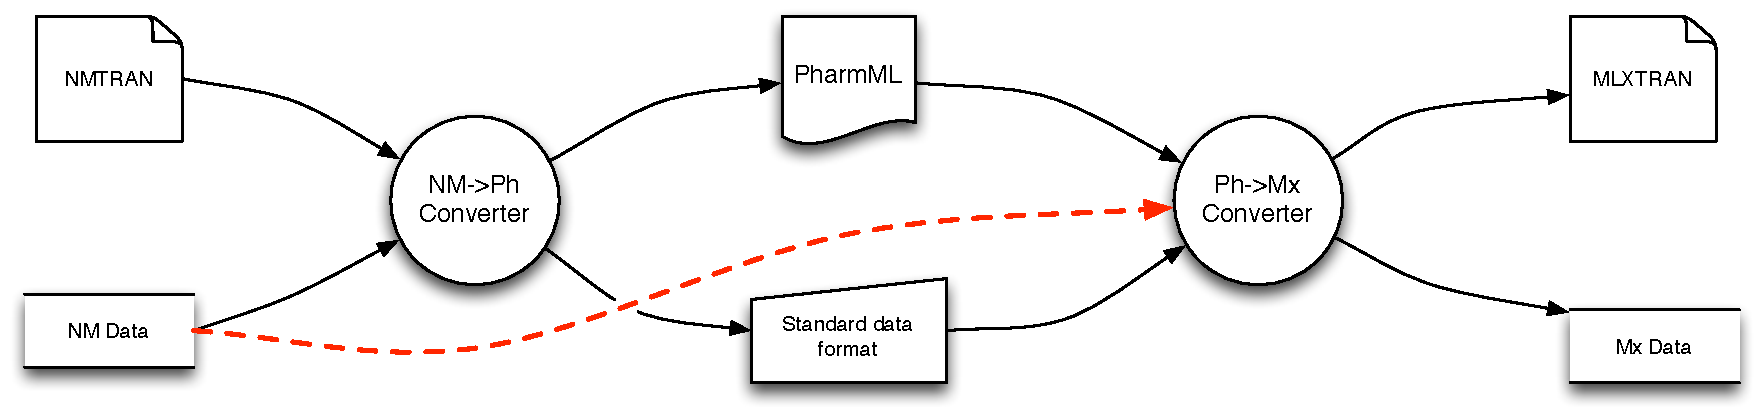
\includegraphics[width=\linewidth]{DataConversion}
\caption{Converting model and data to \pharmml. The figure shows how
  the NONMEM to \pharmml (NM$\rightarrow$Px) converter must convert both the
  model and data and then the \pharmml to MONOLIX (Ph$\rightarrow$Mx) converter
  must convert the \pharmml and standard data files to the MLXTRAN and a
  MONOLIX formatted data file.}
\label{fig:data-conversion}
\end{figure}

This approach undoubtedly requires more work on the part of the
converter generating \pharmml because it must also do the data format
conversion too. However, I would argue that this makes sense because
the developer and maintainer of this converter will of necessity be
very familiar with the tool and so will be familiar with its data
format. Without converting to the standard data format then the
situation illustrated by the red line in figure \ref{fig:data-conversion}
will occur. Here the converter that translates from \pharmml will need
to understand NONMEM data format and convert it into MONOLIX data
format. However, this converter would also need to be able to convert
CVS, TSV, and WinBugs formats too. Clearly this is a lot of work and
it is unlikely that the development and maintenance team will be
closely familiar with these formats. By converting to a standard data
format, however, we can avoid these problems and we can focus our
efforts on providing a software library to wrote and read this
format.

If we wish to adopt a standard data format, what should it be? We
could design our own, but it would make sense to use an existing
standard that is designed for this purpose. My candidate is
NuML\footnote{\url{http://http://code.google.com/p/numl/}}. This
originated from a Systems Biology related format (SBRML) that was
designed to store the results of a simulation\footnote{See also:
  \url{http://www.comp-sys-bio.org/tiki-index.php?page=SBRML}}. It
will hold the tabular data we wish to use for estimation in \pharmml,
but it should also be able to store results generated by estimation
and simulations defined in \pharmml. Since capturing the results of
such tasks is within the scope of \pharmml this allows us to
standardise on one data format for all our needs. Software support is
available in C++ and Java (not native Java) too and there is an XML
Schema that we would be able to reuse directly within \pharmml. We
could therefore embed NuML data directly in the \pharmml file or link
to it as an external file.

\subsection{Units}

A restricted version of the SBML approach looks like it should work in
\pharmml. The question is should we add in units now? The approach
would be to have a built-in set of fundamental units that cover all
dimensions. Then you could define specific units based on these
conventions. For example we may have a $g$ as the fundamental unit of
mass and then define a $kg$ which is a gram scaled by 1000. An example
of what it might look like is below:
%
\begin{xmlcode}
<UnitDefinition symbId="hour">
    <Symbol>h</Symbol>
    <Unit basicUnit="second">
        <Exponent>1</Exponent>
        <Scale>1</Scale>
        <Multiplier>60</Multiplier>
    </Unit>
</UnitDefinition>
\end{xmlcode}
%
The \xelem{UnitDefinition} element defines the unit in terms of a base
unit referred to in the \xelem{Unit} element. Following advice from
Sarah Keating of the SBML team, and the developer who has implemented
unit checking in libSBML, we should keep the set of basic units as
minimal as possible. In this example the idea would be to use the
seven base units from SI\footnote{See Section 2 in
  \url{http://http://www.bipm.org/utils/common/pdf/si_brochure_8.pdf}.}.
The \xelem{Unit} element describes the conversion of the base
unit a consistent of the unit being defined. In this case the unit \emph{hour} is defined
as 60 seconds.

More complex units can contain multiple \xelem{Unit}
elements:
%
\begin{xmlcode}
<UnitDefinition symbId="velocity">
    <ct:Symbol>ms-1</ct:Symbol>
    <Unit basicUnit="metre">
        <Exponent>1</Exponent>
    </Unit>
    <Unit basicUnit="second">
        <Exponent>-1</Exponent>
    </Unit>
</UnitDefinition>
\end{xmlcode}

Above we define velocity, $ms^{-1}$. Note that if the \xelem{Scale}
and \xelem{Multiplier} elements are omitted they are assumed to be
1. The example below shows how we might use these definitions, for
example to define the time units used in the model:
%
\begin{xmlcode}
<IndependentVariable symbId="t">
    <Units symbId="hour"/>
</IndependentVariable>
\end{xmlcode}

Our advice is that the key thing is to put units on all quantities,
including numbers, that was unit consistency checking should be
straightforward as then no inference is required. \pharmml already has
a type system which we need to check for consistency anyway. This
helps here, because units can be thought of as another set of types
and so we should be able to extend the type checking system to
validate unit consistency. My suggestion would be to put in the
structures we need for units now, but only add validation rules about
unit consistency checking later.

\section{Larger Strategic Questions}

% \subsection{Use UncertML 3.0}

% We should start using UncertML 3.0. I think this is
% uncontroversial. We should have a prototype by the end of June that
% will be suitable for inclusion in \pharmml. We should add this in. The
% current Uncertainty.xsd schema used in the current spec was designed
% as a stop-gap until \uncertml was ready. It should be relatively
% painless to swap one in and the other out.

\subsection{Should we adopt MathML for maths?}

In the current spec we use our own mathematical definition for
mathematical equations. This goes against the tide of received opinion
in the Systems Biology world where standards such as CellML and SBML
use variants of MathML. I made a detailed argument in the spec why we
made this decision and for convenience I'll provide this below.

\begin{quotation}
Mathematical equations are a fundamental part of a pharmacometric
model and so it was important that \pharmml incorporated this
ability. The question we had in designing the language, however, was
what is the best way to do this?  Our initial approach was to reuse an
existing W3C standard called
\mathml\footnote{\url{http://www.w3.org/TR/MathML3/}}, which was
designed to represent mathematical equations on web pages.
Unfortunately, the full \mathml standard is bigger and more complex
than we need: indeed much of the standard focuses on the presentation
and layout of mathematical equations rather than their underlying
meaning\footnote{We should emphasise that his is not a criticism of
  \mathml, as this was the problem it was created to solve!}.  This
was the conclusion arrived at similar standards to \pharmml such as
SBML,
CellML\footnote{\url{http://www.cellml.org/specifications/cellml_1.1/\#sec_mathematics}}
and \sedml. Their solution to this problem was to use
a subset of the standard that did what they want and to develop their
own software to support this subset. In effect they created their own
version of the \mathml standard. This means that the CellML version of
\mathml is not compatible with the \sbml version and so on, and as a
consequence each standard has had to develop its own software
libraries to support their own version of \mathml.

Faced with the same dilemma we considered adopting yet another subset
of \mathml, but decided against it for a number of reasons:
\begin{enumerate}
\item Because \mathml is designed for the presentation of maths it's
  basic design is much more complicated that we require.
\item The design of \mathml is such that it is impossible to validate
  whether a sensible mathematical expression has been formed using
  just XML Schema validation\footnote{XML Schema is an XML standard
    that let's you effectively define an object model in XML. The
    benefit of the standard is that it there many tools that can then
    validated automatically whether your XML document conforms to this
    `object model'. We have taken advantage of this technology in
    \pharmml and it has made development of the specification and
    software support much more efficient.}. This is because it uses
  \verb|<apply></apply>| elements to group operands and operators
  together and so a statement such as
  \begin{verbatim}
<apply><divide/><cn>20/<cn></apply>
\end{verbatim}
 (equivalent to $\div 20$) is syntactically valid \mathml, but is an incomplete mathematical
  expression.
\item Taking a subset of \mathml requires the creation of a new XML
  Schema definition, new tools for validation and is effectively
  creating a new standard. In our view calling this \mathml is
  misleading as each of the \mathml subsets currently used are not the
  same and cannot be exchanged with each other, nor with W3C \mathml
  (see discussion above).
\end{enumerate}
Consequently we created our own mathematics definition, which has the
following design goals:
\begin{enumerate}
\item Have a design that ensured that mathematical expressions
  were syntactically correct --- allowing us to use XML Schema
  validating software to ensure this correctness.
\item Ensure that the maths could handle all mathematical expressions
  we require in \pharmml.
\item Provide logical expressions such as in an SQL WHERE, for use in
  datasets for example.
\item Have a simple and concise design that could be easily written by hand
  and also read by a developer --- to facilitate testing.
\end{enumerate}
\end{quotation}

I still hold to these views. The only reason I can see for using
\mathml at all is if we want to encode the maths in \pharmml so that
it can be displayed. There are two places we might want to do
this. The first is in an equation where we could incorporate
presentation and content \mathml. For example:

\begin{xmlcode}
<semantics>
  <mrow>
    <mrow><mo>(</mo><mi>a</mi> <mo>+</mo> <mi>b</mi><mo>)</mo></mrow>
    <mo>&#x2062;<!--INVISIBLE TIMES--></mo>
    <mrow><mo>(</mo><mi>c</mi> <mo>+</mo> <mi>d</mi><mo>)</mo></mrow>
  </mrow>
  <annotation-xml encoding="MathML-Content">
    <apply><and/>
      <apply><xor/><ci>a</ci> <ci>b</ci></apply>
      <apply><xor/><ci>c</ci> <ci>d</ci></apply>
    </apply>
  </annotation-xml>
</semantics>
\end{xmlcode}

The above example (from the \mathml
specification\footnote{url{http://http://www.w3.org/TR/MathML3/}})
encodes the expression $(a+b)(c+d)$ in presentation maths (which is
what would be displayed) but the underlying meaning is the Boolean
expression $(a \text{ AND } b) \text{ OR } (c \text{ AND } d)$. This
is perhaps not the most helpful example, but it shows how the
presentation and meaning can be combined.

Another use of presentation \mathml would be when writing variable
names. Currently variable or parameter names then to be plain text
equivalents forms of mathematical symbols such as \texttt{omega\_V}
for $\omega_V$. Clearly the plain text form is essential in \pharmml
because these names are often used as symbol identifiers. However, it
would be nice to have the mathematical form of a variable or paramater
name encoded in \pharmml so it could be used when the model encoded in
a \pharmml document is presented to user. One way of doing this would
be to use the \xelem{Symbol} element and presentation \mathml as
follows:

\begin{xmlcode}
<Variable symbId="omega_V">
    <Symbol>
        <msub>
            <!-- omega character -->
            <mi>&#x03C9;</mi>
            <mi>V</mi>
        </msub>
    </Symbol>
</Variable>
\end{xmlcode}

Here the \xelem{Symbol} element contains \mathml presentation markup
that would render as $\omega_V$. Of course an alternative would be to
use some other mathematical markup here, such as \LaTeX:

\begin{xmlcode}
<Variable symbId="omega_V">
    <Symbol>\omega_V</Symbol>
</Variable>
\end{xmlcode}

The benefit of using presentation \mathml is that most web browsers
and a number of maths related software would recognise the
presentation markup and display it. When combined with content \mathml
this would in theory provide one encoding that would provide both a
visual and semantic representation of the maths.

The downside of this approach is undoubtedly complexity. \mathml is
much bigger than we need because it can be used to describe complete
equations (we only need to define the RHS of an equation), with
matrices and symbols that we do not require. In addition it is not
clear if there are software libraries we could reuse to help parse and
validate the \mathml content.

This really is a open question. My biais is to use our own maths
representation rather than use a subset of \mathml. However, if we are
starting to think about presenting the maths encoded in \pharmml then
it may make more sense to adopt \mathml (in its entirety) to do this
--- after all this is what \mathml is designed to do.

% \subsection{Should we drop the Trial Design section?}

% Currently we have the ability to define the design of a Clinical Trial
% which has multiple groups/arms each containing multiple treatments. We
% can do trials with wash-outs between sets of treatments and we can
% defining multiple types of drug administration: bolus and
% infusion. Within periods of treatment (which we call the treatment
% epoch) we can define occasions which are typically used to indicate
% that there was a source of variability in the taking of observations
% from the patients in a given treatment group. This means we can define
% a large subset of clinical trials using this approach and we can also
% define trials with BSV and IOV levels of variability.

% All the above is good and we have shown that it works and can be used
% to make the definition of the trial much clearer. However, at the
% moment this structure does not reflect how software tools define a clinical
% trial used by a model. Typically this is done within a data file,
% where the individuals, occasions, dosing and dosing time points are
% all specified. We also support this approach.

% However, at the moment the Trail Design section of \pharmml
% is unlikely to be used `out in the wild'. MCL does not support it so
% the WP2 infrastructure will not generate \pharmml models that use
% it. Neither NONMEM nor MONOLIX have this information defined
% explicitly so again \pharmml documents generated from these tools will
% be unlikely to define the trial design in this section.

% As has been said, the Trial Design section currently defines a subset
% of trials designs. There is a significant risk that our current design
% will be too limiting to be able to define all possible trial
% designs. If this is the case then we may have an issue where at a
% future date we need to completely redesign this part of \pharmml. This
% redesign may be significantly more complex than our current design. If
% it is then are we clear that there is benefit in maintaining a
% complex representation that is never used by tools?

% Finally, I think we should think hard about why we are defining the
% trial design like this? If this is not the way the field currently
% defines clinical trials in models are we aspiring to lead the field
% and encourage tools to adopt a new way of doing things? If this is our
% aim is that an appropriate one? Perhaps we should be focusing on what is
% standard practise in the field as it is?

% I am undecided about this, but I am inclining to the view that we
% should focus on the data-driven approaches and drop the Trial Design
% section from the public release. We can still work on it (as a lower
% priority) and it may be something we can re-introduce at a later
% date. By that time our greater experience and the greater credibility
% of \pharmml as it becomes more widely used may enable us to have a
% better idea of the limitations of our current approach and also may
% make the users of \pharmml more receptive to our approach for explicit
% trial design.

\section{For consideration}

Here I've put changes that we may need to make or at least consider,
but for which I don't have a proposed solution.

\subsection{Support for multi-variate distributions}

Currently \pharmml does not support multivariate distributions. We can
define correlated random variables which are in effect multivariate
normal distributions, but we cannot define them explicitly. I know
that Mike Smith advocates that we should do so and MDL has explicit
support for multivariate distributions.

To support this requires at the very least support for arrays and
possibly matrices. This may also mean that we need to be able to have
matrix/array operators as they do in Matlab. If we need to do this
then we should consider it carefully because the knock-on effects are
potentially significant. That said the design of the current
spec and the spec with the changes proposed here applied is flexible
enough to permit us to add such features and maintain compatibility
with previous versions. We should assess whether we need multivariate
distributions and in particular whether we can be compatible with MDL
without them. If we can then I suggest we postpone their addition
until a later release.

\subsection{Reset Type}

We have a Washout Type which resets the dose, and structural model
variables back to their initial values. Perhaps we should define a
reset element that resets some variables to zero. We should investigate
the approach used by NONMEM. We probably need this
functionality to have maximum flexibility. I have no proposal on how
to do this, however.



\end{document}
